\subsection{Hyper-Parameter Tuning Protocol}\label{sec:tuning-protocol}

In all our experiments, we tune the following optimizer hyper-parameters and otherwise use the PyTorch default values:
\begin{itemize}
\item \textbf{SGD:} learning rate, momentum
\item \textbf{Adam:} learning rate
\item \textbf{Hessian-free:} type of curvature matrix (Hessian or GGN), damping, whether to adapt damping over time (yes or no), maximum number of CG iterations
\item \textbf{LBFGS:} learning rate, history size
\item \textbf{ENGD:} damping, factor of the exponential moving average applied to the Gramian, initialization of the Gramian (zero or identity matrix)
\item \textbf{KFAC:} factor of the exponential moving average applied to the Kronecker factors, damping, momentum, initialization of the Kronecker factors (zero or identity matrix)
\item \textbf{KFAC*:} factor of the exponential moving average applied to the Kronecker factors, damping, initialization of the Kronecker factors (zero or identity matrix)
\end{itemize}

Depending on the optimizer and experiment we use grid, random, or Bayesian search from Weights \& Biases.
Each individual run is allowed to run for a given time budget, and the best run within a search is given by that with lowest final $L_2$ error on a fixed evaluation data set.
All runs are executed on RTX 6000 GPUs with 24\,GiB of RAM to be comparable.
For grid and random searches, we use a round-based approach.
First, we choose a relatively wide search space and limit to approximately 50 runs.
In a second, round, we narrow down the hyper-parameter space based on the first round, then re-run for another approximately 50 runs.
We will release the details of all hyper-parameter search spaces, as well as the hyper-parameters for the best runs in our implementation.

\subsection{Two-dimensional Poisson Equation}

We consider a two-dimensional Poisson equation $\Delta u(x, y) = 2 \pi^2 \sin(\pi x) \sin(\pi y)$ on the unit square $(x,y) \in [0, 1]^2$ with sine product right hand side and zero boundary conditions $u(x, y) = 0$ for $(x,y) \in \partial [0,1]^2$.
We choose a single set of training points with $N_{\Omega} = 900, N_{\partial\Omega} = 120$.
The $L_2$ error is evaluated on a separate set of $\num{9000}$ data points.
Each run is limited to 1000\,s.
We compare three MLP architectures of increasing size, each of whose linear layers are Tanh-activated except for the final one: a shallow $2\to64\to1$ MLP with $D=257$, a five layer $2 \to 64 \to 64 \to 48 \to 48 \to 1$ MLP with $D=\num{9873}$, and a five layer $2 \to 256 \to 256\to 128 \to 128 \to 1$ MLP with $D=\num{116097}$.
For the biggest architecture, ENGD-full leads to out-of-memory errors.
Figure~\Cref{fig:poisson2d-appendix} visualizes the best runs:
\begin{itemize}
  \def\pathToRuns{../kfac_pinns_exp/exp09_reproduce_poisson2d/tex}
\item \textbf{SGD:} learning rate: $\num[scientific-notation=true]{3.758303e-03}$, momentum: $\num[scientific-notation=true]{0.9}$
\item \textbf{Adam:} learning rate: $\num[scientific-notation=true]{6.406108e-04}$
\item \textbf{Hessian-free:} curvature matrix: GGN, initial damping: 100, constant damping: no, maximum CG iterations: 50
\item \textbf{LBFGS:} learning rate: $\num[scientific-notation=true]{0.1}$, history size: 200
\item \textbf{ENGD (full):} damping: $\num[scientific-notation=true]{1e-10}$, exponential moving average: $\num[scientific-notation=true]{0.3}$, initialize Gramian to identity: yes
\item \textbf{ENGD (layer-wise):} damping: 0, exponential moving average: $\num[scientific-notation=true]{0.9}$, initialize Gramian to identity: yes
\item \textbf{KFAC} damping: $\num[scientific-notation=true]{2.640390e-11}$, momentum: $\num[scientific-notation=true]{9.995595e-02}$, exponential moving average: $\num[scientific-notation=true]{5.556664e-01}$, initialize Kronecker factors to identity: yes
\item \textbf{KFAC*} damping: $\num[scientific-notation=true]{2.989247e-13}$, exponential moving average: $\num[scientific-notation=true]{6.258340e-01}$, initialize Kronecker factors to identity: yes
\end{itemize}

\begin{figure}[!h]
  \centering
  \begin{subfigure}[t]{1.0\linewidth}
    \caption{}\label{subfig:poisson2d-time}
    % trim legend, xlabel and xticklabels
    % [trim={left bottom right top},clip]
    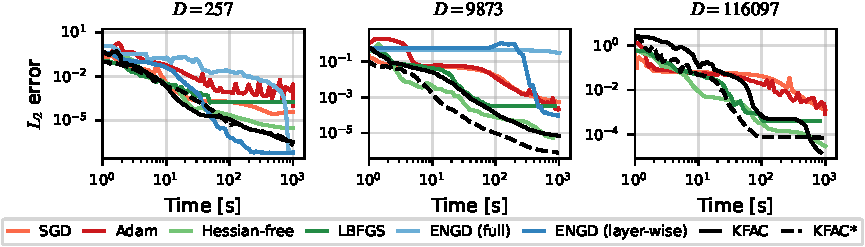
\includegraphics[trim={0 1.3cm 0 0},clip]{../kfac_pinns_exp/exp17_groupplot_poisson2d/l2_error_over_time.pdf}
    % trim the legend and titles
    % [trim={left bottom right top},clip]
    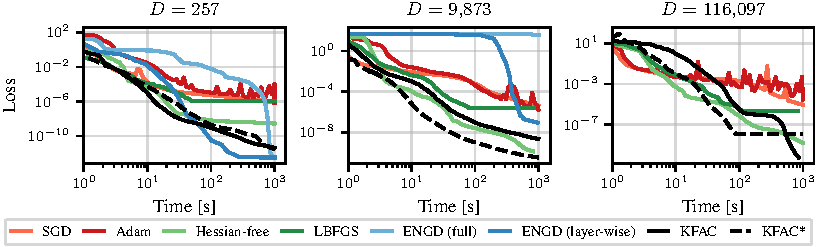
\includegraphics[trim={0 0.5cm 0 0.3cm},clip]{../kfac_pinns_exp/exp17_groupplot_poisson2d/loss_over_time.pdf}
  \end{subfigure}
  \begin{subfigure}[t]{1.0\linewidth}
    \caption{}\label{subfig:poisson2d-step}
    % trim the legend, xlabel and xticklabels
    % [trim={left bottom right top},clip]
    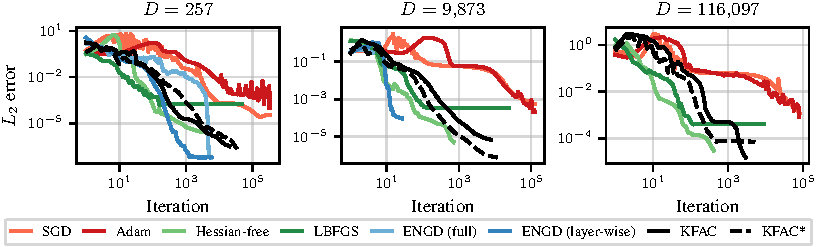
\includegraphics[trim={0 1.3cm 0 0.3cm},clip]{../kfac_pinns_exp/exp17_groupplot_poisson2d/l2_error_over_step.pdf}
    % trim the titles
    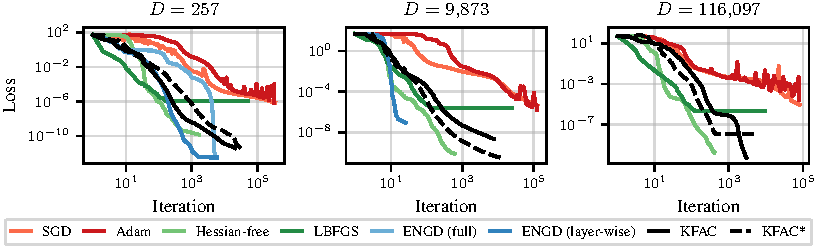
\includegraphics[trim={0 0 0 0.3cm},clip]{../kfac_pinns_exp/exp17_groupplot_poisson2d/loss_over_step.pdf}
  \end{subfigure}
  \caption{ Training loss and evaluation $L_2$ error for learning the solution to a 2d Poisson equation over (\subref{subfig:poisson2d-time}) time and (\subref{subfig:poisson2d-step}) steps.
    Column are different neural networks.}\label{fig:poisson2d-appendix}
\end{figure}

\clearpage

\subsection{Five-dimensional Poisson Equation}

\begin{figure}[!h]
  \centering
  % 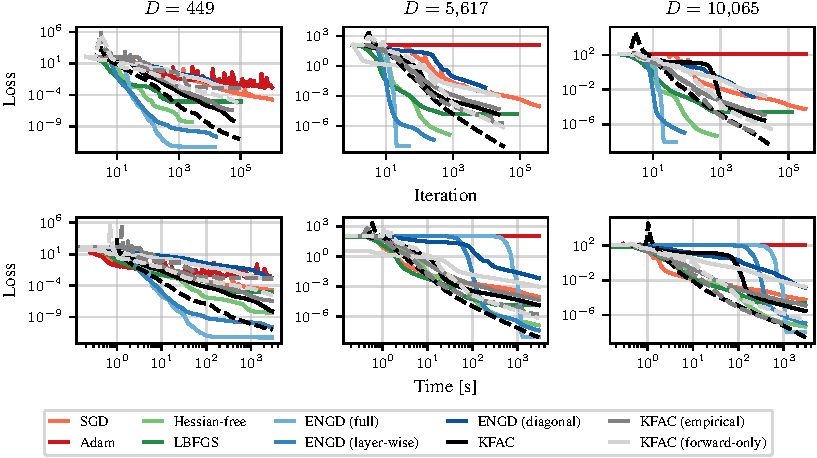
\includegraphics{../kfac_pinns_exp/exp18_groupplot_poisson5d/loss_all.pdf}
  % \\
  % 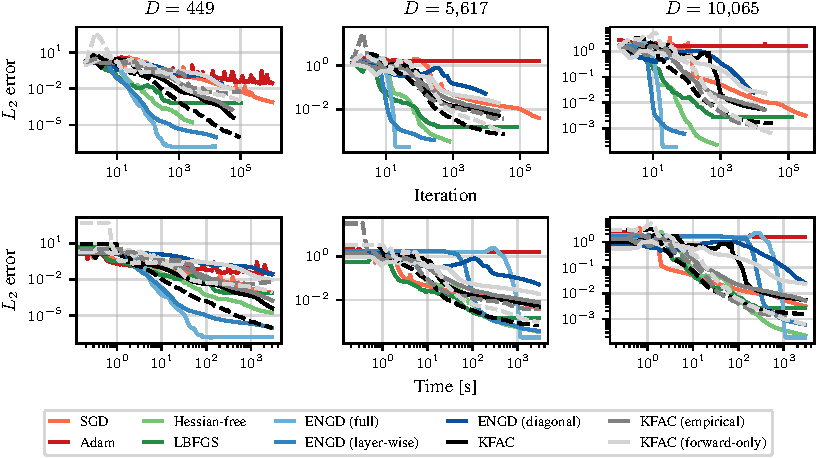
\includegraphics{../kfac_pinns_exp/exp18_groupplot_poisson5d/l2_error_all.pdf}
  \caption{Loss curves for learning the solution of a 5d-Poisson equation with different neural network size under a given time budget of $3\cdot 10^3\,\text{s}$ on an RTX 6000 GPU.
    Top row shows loss over time, bottom row shows loss over step.}
\end{figure}

%%% Local Variables:
%%% mode: latex
%%% TeX-master: "../main"
%%% End:
